\chapter{Related work}
\section{Boundary attack}
\gls{ba} \cite{boundary_attack} is a decision-based adversarial attack. The basic intuition of \gls{ba} differs from traditional adversarial attacks. Unlike these traditional adversarial attacks, where the original image is moved through search space in order to become adversarial, \gls{ba} starts from an input that is already adversarial. This input is then moved closer to the original image, while staying adversarial.\\

The attack has to be initialized with an already adversarial input. Two different approaches can be taken depending on the attack setting. In the untargeted case, the input can be sampled from a maximum entropy distribution given the valid domain of this input. Samples that are not adversarial are rejected. An example of such a starting position can be seen in Figure \ref{fig:uniform_noise}. In the case of a targeted attack, the input is a sample from the dataset that is classified as the target class by the model under attack.\\

\gls{ba} iteratively updates the adversarial image by performing a step orthogonal to the original image and a step towards this image. In iteration $k$, a perturbation $\eta_k$ is sampled from a uniform distribution. This perturbation is rescaled and added to the adversarial image. From this new position in search space, the step towards the original image is taken. This way the path of the attack follows the decision boundary, hence the name of the attack. The intuition of the \gls{ba} is shown in Figure~\ref{fig:boundary_attack_intuition}. The attack can only follow the boundary if the adversarial image is already near the boundary. The starting image is projected onto the boundary using binary search to ensure that the adversarial image is in the vicinity of the boundary.\\

The step sizes are adjusted according to local geometry of the boundary. The orthogonal step size $\delta$ is adjusted so that approximately half of the orthogonal perturbations is still adversarial. This approach is based on trust region methods \cite{trm}. The step size towards the original image $\epsilon$ is adjusted using the same principle, but here a user specified threshold is used. The decision boundary tends to become flatter, the closer to the original image the attack gets \cite{straight_boundaries}. Therefore the algorithm converges when $\epsilon$ converges to zero.\\

\gls{bba} \cite{brunner_guessing_2019} (previously known as \textit{Boundary Attack++}) is an improvement on the original \gls{ba} in three different ways. All three improvements will be discussed in order of the strength of their effect. The first improvement is a biased sampling technique. The key idea behind this strategy is that most previous attacks yield adversarial examples with high frequencies in the image. By sampling the perturbations in the first step of the \gls{ba} from a low frequency distribution, the frequency of the created adversarial example will be lowered as well. \gls{bba} does this by sampling from a Perlin noise \cite{perlin} distribution instead of a uniform distribution. Lower frequency images yield more natural results and can more easily bypass simple preprocessing defense schemes. The difference between the two noise patterns can be seen in Figure \ref{fig:noise_differences}. The noise patterns can be influenced by a frequency value. This value can be tuned depending on the size of the images at hand. Higher frequency values yield less smooth noise patterns. Figure \ref{fig:perlin_noise_frequencies} visually shows the influence of the frequency values.\\

\begin{figure}
	\centering
	\subfloat[Uniform noise]{%
	\label{fig:uniform_noise}%
	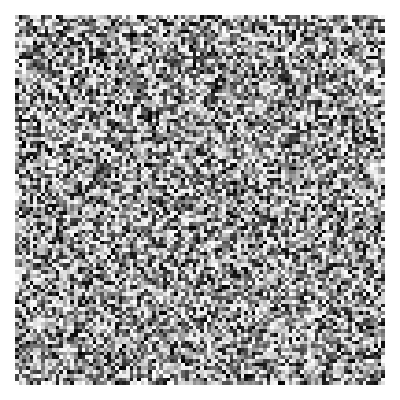
\includegraphics[width=.4\linewidth]{Images/gaussian_noise}
	}\qquad
	\subfloat[Perlin noise]{%
	\label{fig:perlin_noise}%
	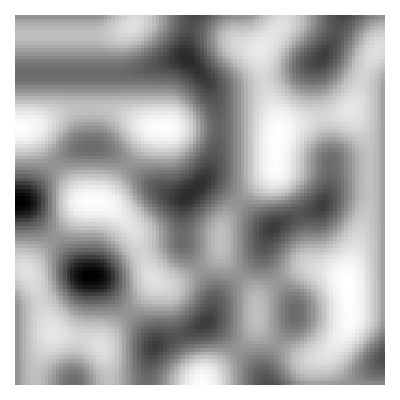
\includegraphics[width=.4\linewidth]{Images/perlin_noise}
	}
	\caption[Difference between noise patterns]{Difference between noise patterns.}
	\label{fig:noise_differences}
\end{figure}

\begin{figure}
	\centering
	\subfloat[Frequency 2]{%
	\label{fig:perlin_noise_2}%
	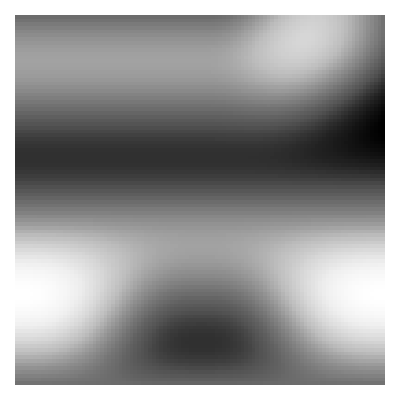
\includegraphics[width=.3\linewidth]{Images/perlin_noise_2}
	}\quad
	\subfloat[Frequency 5]{%
	\label{fig:perlin_noise_5}%
	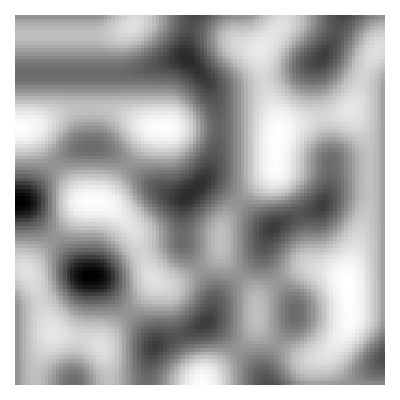
\includegraphics[width=.3\linewidth]{Images/perlin_noise}
	}\quad
	\subfloat[Frequency 20]{%
	\label{fig:perlin_noise_20}%
	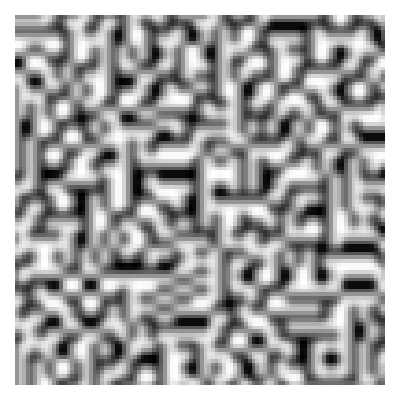
\includegraphics[width=.3\linewidth]{Images/perlin_noise_20}
	}
	\caption[Influence of frequency on Perlin noise]{Influence of frequency on Perlin noise patterns.}
	\label{fig:perlin_noise_frequencies}
\end{figure}

The second improvement is to use a regional mask. The original \gls{ba} applies a perturbation to the images as a whole. Every pixel will be perturbed with the same magnitude. This magnitude can be altered on a per-pixel basis when using a mask. Pixels that are further away from the target image will receive a larger perturbation than pixels that are already close to the corresponding pixel in the target. The mask $m$ is constructed according to equation \ref{eq:mask} based on the original image $x_{orig}$ and the adversarial image $x_{adv}$. It is then pixel-wise applied to the sampled perturbation in equation \ref{eq:mask_app}. The masked perturbation is normalized afterwards.\\ 

\begin{align}
m &= | x_{adv} - x_{orig}| \label{eq:mask}\\
\eta_{k} &= m \odot \eta_k; \eta_k = \frac{\eta_k}{\| \eta_k \|} \label{eq:mask_app}
\end{align}

This technique improves efficiency since the search space is significantly reduced. It is also possible to engineer masks for specific examples in order to incorporate other knowledge in the attack.\\

The final improvement is based on the idea of transfer attacks. A surrogate model is trained and will be used to calculate adversarial gradients. These gradients will then be used to bias the sampling direction for the orthogonal step. If the surrogate model does not closely resemble the defender, then the gradients will only hamper the speed of convergence of the attack instead of causing the attack to fail.

\begin{figure}
\centering
\tikzset{every picture/.style={line width=0.75pt}} %set default line width to 0.75pt        
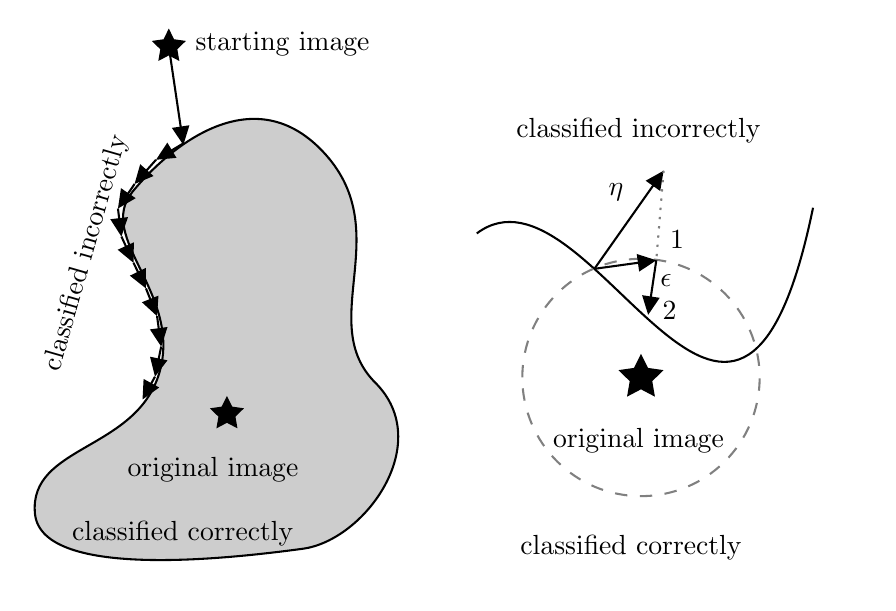
\begin{tikzpicture}[x=0.75pt,y=0.75pt,yscale=-1,xscale=1]
%uncomment if require: \path (0,300); %set diagram left start at 0, and has height of 300

%Shape: Polygon Curved [id:ds5185908380685693] 
\draw  [fill={rgb, 255:red, 155; green, 155; blue, 155 }  ,fill opacity=0.5 ] (77.12,91.56) .. controls (95.12,69.56) and (136.12,35.56) .. (170.12,73.56) .. controls (204.12,111.56) and (165.12,154.56) .. (194.12,183.56) .. controls (223.12,212.56) and (189.12,259.56) .. (159.12,263.56) .. controls (129.12,267.56) and (33.12,279.56) .. (30.12,246.56) .. controls (27.12,213.56) and (79.12,216.56) .. (90.12,178.56) .. controls (101.12,140.56) and (59.12,113.56) .. (77.12,91.56) -- cycle ;
%Shape: Star [id:dp7170747564600322] 
\draw  [fill={rgb, 255:red, 0; green, 0; blue, 0 }  ,fill opacity=1 ] (122.62,191.06) -- (124.83,195.53) -- (129.76,196.24) -- (126.19,199.72) -- (127.03,204.63) -- (122.62,202.31) -- (118.22,204.63) -- (119.06,199.72) -- (115.49,196.24) -- (120.42,195.53) -- cycle ;
%Shape: Star [id:dp10477759386916752] 
\draw  [fill={rgb, 255:red, 0; green, 0; blue, 0 }  ,fill opacity=1 ] (94.62,14.06) -- (96.83,18.53) -- (101.76,19.24) -- (98.19,22.72) -- (99.03,27.63) -- (94.62,25.31) -- (90.22,27.63) -- (91.06,22.72) -- (87.49,19.24) -- (92.42,18.53) -- cycle ;
%Straight Lines [id:da2531323347021954] 
\draw    (94.62,21.56) -- (101.19,66.01) ;
\draw [shift={(101.62,68.98)}, rotate = 261.6] [fill={rgb, 255:red, 0; green, 0; blue, 0 }  ][line width=0.08]  [draw opacity=0] (8.93,-4.29) -- (0,0) -- (8.93,4.29) -- cycle    ;
%Straight Lines [id:da6594852147606747] 
\draw    (101.79,68.14) -- (91.03,74.6) ;
\draw [shift={(88.46,76.14)}, rotate = 329.04] [fill={rgb, 255:red, 0; green, 0; blue, 0 }  ][line width=0.08]  [draw opacity=0] (8.93,-4.29) -- (0,0) -- (8.93,4.29) -- cycle    ;
%Straight Lines [id:da6002841525279263] 
\draw    (88.46,76.14) -- (80.11,85.56) ;
\draw [shift={(78.12,87.81)}, rotate = 311.53] [fill={rgb, 255:red, 0; green, 0; blue, 0 }  ][line width=0.08]  [draw opacity=0] (8.93,-4.29) -- (0,0) -- (8.93,4.29) -- cycle    ;
%Straight Lines [id:da9148455444041863] 
\draw    (78.12,87.81) -- (71.8,97.16) ;
\draw [shift={(70.12,99.64)}, rotate = 304.06] [fill={rgb, 255:red, 0; green, 0; blue, 0 }  ][line width=0.08]  [draw opacity=0] (8.93,-4.29) -- (0,0) -- (8.93,4.29) -- cycle    ;
%Straight Lines [id:da47669503735159546] 
\draw    (70.12,99.64) -- (71.42,110.17) ;
\draw [shift={(71.79,113.14)}, rotate = 262.96] [fill={rgb, 255:red, 0; green, 0; blue, 0 }  ][line width=0.08]  [draw opacity=0] (8.93,-4.29) -- (0,0) -- (8.93,4.29) -- cycle    ;
%Straight Lines [id:da26104674623686774] 
\draw    (71.79,113.14) -- (76.37,123.08) ;
\draw [shift={(77.62,125.81)}, rotate = 245.27] [fill={rgb, 255:red, 0; green, 0; blue, 0 }  ][line width=0.08]  [draw opacity=0] (8.93,-4.29) -- (0,0) -- (8.93,4.29) -- cycle    ;
%Straight Lines [id:da9792015265988265] 
\draw    (77.62,125.81) -- (82.31,135.45) ;
\draw [shift={(83.62,138.14)}, rotate = 244.06] [fill={rgb, 255:red, 0; green, 0; blue, 0 }  ][line width=0.08]  [draw opacity=0] (8.93,-4.29) -- (0,0) -- (8.93,4.29) -- cycle    ;
%Straight Lines [id:da8018833944649997] 
\draw    (83.62,138.14) -- (87.84,148.69) ;
\draw [shift={(88.96,151.48)}, rotate = 248.2] [fill={rgb, 255:red, 0; green, 0; blue, 0 }  ][line width=0.08]  [draw opacity=0] (8.93,-4.29) -- (0,0) -- (8.93,4.29) -- cycle    ;
%Straight Lines [id:da7469050329272713] 
\draw    (88.96,151.48) -- (90.55,163.17) ;
\draw [shift={(90.96,166.14)}, rotate = 262.23] [fill={rgb, 255:red, 0; green, 0; blue, 0 }  ][line width=0.08]  [draw opacity=0] (8.93,-4.29) -- (0,0) -- (8.93,4.29) -- cycle    ;
%Straight Lines [id:da36931886382540347] 
\draw    (90.96,166.14) -- (88.57,177.7) ;
\draw [shift={(87.96,180.64)}, rotate = 281.69] [fill={rgb, 255:red, 0; green, 0; blue, 0 }  ][line width=0.08]  [draw opacity=0] (8.93,-4.29) -- (0,0) -- (8.93,4.29) -- cycle    ;
%Straight Lines [id:da3125285737899821] 
\draw    (87.96,180.64) -- (83.39,189.01) ;
\draw [shift={(81.96,191.64)}, rotate = 298.61] [fill={rgb, 255:red, 0; green, 0; blue, 0 }  ][line width=0.08]  [draw opacity=0] (8.93,-4.29) -- (0,0) -- (8.93,4.29) -- cycle    ;

%Curve Lines [id:da7332610230112269] 
\draw    (243,111.62) .. controls (297.92,70.43) and (367.93,279.11) .. (405,99.26) ;
%Shape: Star [id:dp6998768571531213] 
\draw  [fill={rgb, 255:red, 0; green, 0; blue, 0 }  ,fill opacity=1 ] (322.11,170.74) -- (325.14,176.87) -- (331.9,177.85) -- (327.01,182.62) -- (328.16,189.36) -- (322.11,186.18) -- (316.06,189.36) -- (317.22,182.62) -- (312.32,177.85) -- (319.09,176.87) -- cycle ;
%Straight Lines [id:da9467918607674688] 
\draw    (299.68,128.68) -- (331.29,83.87) ;
\draw [shift={(333.02,81.42)}, rotate = 125.2] [fill={rgb, 255:red, 0; green, 0; blue, 0 }  ][line width=0.08]  [draw opacity=0] (8.93,-4.29) -- (0,0) -- (8.93,4.29) -- cycle    ;
%Shape: Ellipse [id:dp07084957668985581] 
\draw  [color={rgb, 255:red, 128; green, 128; blue, 128 }  ,draw opacity=1 ][dash pattern={on 4.5pt off 4.5pt}] (264.94,181.03) .. controls (264.94,149.46) and (290.54,123.86) .. (322.11,123.86) .. controls (353.69,123.86) and (379.28,149.46) .. (379.28,181.03) .. controls (379.28,212.61) and (353.69,238.2) .. (322.11,238.2) .. controls (290.54,238.2) and (264.94,212.61) .. (264.94,181.03) -- cycle ;
%Straight Lines [id:da7547924674466151] 
\draw    (299.68,128.68) -- (326.52,124.97) ;
\draw [shift={(329.49,124.56)}, rotate = 172.13] [fill={rgb, 255:red, 0; green, 0; blue, 0 }  ][line width=0.08]  [draw opacity=0] (8.93,-4.29) -- (0,0) -- (8.93,4.29) -- cycle    ;
%Straight Lines [id:da7777022216727221] 
\draw    (329.49,124.56) -- (326.01,147.88) ;
\draw [shift={(325.57,150.85)}, rotate = 278.49] [fill={rgb, 255:red, 0; green, 0; blue, 0 }  ][line width=0.08]  [draw opacity=0] (8.93,-4.29) -- (0,0) -- (8.93,4.29) -- cycle    ;
%Straight Lines [id:da931484330606797] 
\draw [color={rgb, 255:red, 128; green, 128; blue, 128 }  ,draw opacity=1 ] [dash pattern={on 0.84pt off 2.51pt}]  (333.02,81.42) -- (329.49,124.56) ;


% Text Node
\draw (328.21,263) node   [align=left] {\begin{minipage}[lt]{96.27pt}\setlength\topsep{0pt}
classified correctly
\end{minipage}};
% Text Node
\draw (326.21,62) node   [align=left] {\begin{minipage}[lt]{96.27pt}\setlength\topsep{0pt}
classified incorrectly
\end{minipage}};
% Text Node
\draw (325.12,211.56) node   [align=left] {\begin{minipage}[lt]{68pt}\setlength\topsep{0pt}
original image
\end{minipage}};
% Text Node
\draw (112.21,256.14) node   [align=left] {\begin{minipage}[lt]{96.27pt}\setlength\topsep{0pt}
classified correctly
\end{minipage}};
% Text Node
\draw (106,13) node [anchor=north west][inner sep=0.75pt]   [align=left] {starting image};
% Text Node
\draw (56.21,116) node  [rotate=-286.01] [align=left] {\begin{minipage}[lt]{96.27pt}\setlength\topsep{0pt}
classified incorrectly
\end{minipage}};
% Text Node
\draw (120.12,225.56) node   [align=left] {\begin{minipage}[lt]{68pt}\setlength\topsep{0pt}
original image
\end{minipage}};
% Text Node
\draw (381.43,114.71) node   [align=left] {\begin{minipage}[lt]{68pt}\setlength\topsep{0pt}
1
\end{minipage}};
% Text Node
\draw (377.9,148.85) node   [align=left] {\begin{minipage}[lt]{68pt}\setlength\topsep{0pt}
2
\end{minipage}};
% Text Node
\draw (330,130) node [anchor=north west][inner sep=0.75pt]   [align=left] {$\displaystyle \epsilon $};
% Text Node
\draw (305,86) node [anchor=north west][inner sep=0.75pt]   [align=left] {$\displaystyle \eta $};


\end{tikzpicture}
\caption[Intuition of the Boundary Attack]{Intuition behind the Boundary Attack. On the left the path of the attack is shown. The first step is a projection onto the boundary, afterwards it follows the decision boundary of the class of the original image. Each arrow represents one iteration of the attack. On the right, the two different steps of each iteration can be seen. In the first step, a random direction is sampled and projected onto a sphere around the original image. The second step is to take a step towards the original image from this new position. Image inspired by \cite{boundary_attack}.}
\label{fig:boundary_attack_intuition}
\end{figure}

\section{HopSkipJumpAttack}
\gls{hsja} \cite{hsja}, like \gls{ba}, is a decision-based adversarial attack that starts from an adversarial input. The initial input is obtained in an identical manner as in \gls{ba}. \gls{hsja} is an iterative algorithm that consists of three steps.\\

The first step is a projection onto the decision boundary of the model under attack. This projection is carried out using a binary search. The second step is to estimate the direction of the gradient at the boundary. Different directions are sampled from a uniform distribution over a $d$-dimensional sphere, where $d$ is the input dimension. This random direction is added to the boundary point, generating a new query for the model. The results of these queries are combined to a gradient estimation~$\widetilde{\nabla S}$ using the Monte Carlo estimate of equation \ref{eq:monte_carlo_estimate}. In this equation $u_b$ are the random directions and $x_t$ is the boundary position. $B$ is the number of random directions that needs to be sampled. This number increases based on the current iteration of the attack to reduce the variance of the estimate. The function~$\phi_{x^*}$ returns 1 if the new position is adversarial and -1 if it is not adversarial. $\delta$ is a positive parameter determining the size of the $d$-dimensional sphere.

\begin{equation}\label{eq:monte_carlo_estimate}
\widetilde{\nabla S}(x_t,\delta) := \frac{1}{B} \sum_{b=1}^{B}\phi_{x^*}(x_t + \delta u_b)u_b
\end{equation}

Once the gradient has been estimated, the third and final operation is to take a step along this gradient. The step size is determined using a geometric progression scheme. These steps are iteratively repeated until the pre-set stopping criterion is met. Figure \ref{fig:hsja_intuition} represents the intuition behind \gls{hsja} in a graphical manner.\\

\gls{hsja} eclipses \gls{ba} and \gls{bba} both on median distance against queries and attack success rates using a limited amount of queries. The untargeted version of \gls{hsja} is able to compete with white box attacks on the ImageNet dataset \cite{imagenet}. It also performs similar or superior to white box attacks such as the C\&W attack \cite{cw_attack} when evaluated against defensive mechanisms such as defensive distillation \cite{defensive_distillation}, region-based classification \cite{region-based_classification} and adversarial training \cite{FGSM}.


\begin{figure}
\centering


\tikzset{every picture/.style={line width=0.75pt}} %set default line width to 0.75pt        

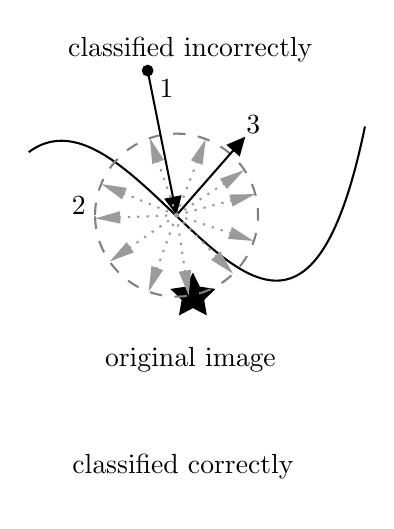
\begin{tikzpicture}[x=0.75pt,y=0.75pt,yscale=-1,xscale=1]
%uncomment if require: \path (0,300); %set diagram left start at 0, and has height of 300

%Curve Lines [id:da9704742483773781] 
\draw    (243,111.62) .. controls (297.92,70.43) and (367.93,279.11) .. (405,99.26) ;
%Shape: Star [id:dp26832364802919195] 
\draw  [fill={rgb, 255:red, 0; green, 0; blue, 0 }  ,fill opacity=1 ] (322.11,170.74) -- (325.14,176.87) -- (331.9,177.85) -- (327.01,182.62) -- (328.16,189.36) -- (322.11,186.18) -- (316.06,189.36) -- (317.22,182.62) -- (312.32,177.85) -- (319.09,176.87) -- cycle ;
%Shape: Ellipse [id:dp9511930412387599] 
\draw  [color={rgb, 255:red, 128; green, 128; blue, 128 }  ,draw opacity=1 ][dash pattern={on 4.5pt off 4.5pt}] (274.97,141.94) .. controls (274.97,120.26) and (292.54,102.69) .. (314.22,102.69) .. controls (335.9,102.69) and (353.48,120.26) .. (353.48,141.94) .. controls (353.48,163.63) and (335.9,181.2) .. (314.22,181.2) .. controls (292.54,181.2) and (274.97,163.63) .. (274.97,141.94) -- cycle ;
%Shape: Circle [id:dp5681517768642557] 
\draw  [fill={rgb, 255:red, 0; green, 0; blue, 0 }  ,fill opacity=1 ] (298,72.3) .. controls (298,71.03) and (299.03,70) .. (300.3,70) .. controls (301.57,70) and (302.6,71.03) .. (302.6,72.3) .. controls (302.6,73.57) and (301.57,74.6) .. (300.3,74.6) .. controls (299.03,74.6) and (298,73.57) .. (298,72.3) -- cycle ;
%Straight Lines [id:da06387380835189371] 
\draw    (300.3,72.3) -- (313.63,139) ;
\draw [shift={(314.22,141.94)}, rotate = 258.7] [fill={rgb, 255:red, 0; green, 0; blue, 0 }  ][line width=0.08]  [draw opacity=0] (8.93,-4.29) -- (0,0) -- (8.93,4.29) -- cycle    ;
%Straight Lines [id:da5011613685801404] 
\draw [color={rgb, 255:red, 155; green, 155; blue, 155 }  ,draw opacity=1 ][line width=0.75]  [dash pattern={on 0.84pt off 2.51pt}]  (314.22,141.94) -- (279.9,127.76) ;
\draw [shift={(278.05,127)}, rotate = 22.45] [fill={rgb, 255:red, 155; green, 155; blue, 155 }  ,fill opacity=1 ][line width=0.08]  [draw opacity=0] (12,-3) -- (0,0) -- (12,3) -- cycle    ;
%Shape: Boxed Line [id:dp5969211465757109] 
\draw [color={rgb, 255:red, 155; green, 155; blue, 155 }  ,draw opacity=1 ][line width=0.75]  [dash pattern={on 0.84pt off 2.51pt}]  (314.22,141.94) -- (327.54,107.28) ;
\draw [shift={(328.26,105.41)}, rotate = 111.02] [fill={rgb, 255:red, 155; green, 155; blue, 155 }  ,fill opacity=1 ][line width=0.08]  [draw opacity=0] (12,-3) -- (0,0) -- (12,3) -- cycle    ;
%Shape: Boxed Line [id:dp06580944891073615] 
\draw [color={rgb, 255:red, 155; green, 155; blue, 155 }  ,draw opacity=1 ][line width=0.75]  [dash pattern={on 0.84pt off 2.51pt}]  (314.22,141.94) -- (350.1,132.34) ;
\draw [shift={(352.03,131.82)}, rotate = 165.01] [fill={rgb, 255:red, 155; green, 155; blue, 155 }  ,fill opacity=1 ][line width=0.08]  [draw opacity=0] (12,-3) -- (0,0) -- (12,3) -- cycle    ;
%Shape: Boxed Line [id:dp5760742560965917] 
\draw [color={rgb, 255:red, 155; green, 155; blue, 155 }  ,draw opacity=1 ][line width=0.75]  [dash pattern={on 0.84pt off 2.51pt}]  (314.22,141.94) -- (340.03,168.65) ;
\draw [shift={(341.42,170.09)}, rotate = 225.98] [fill={rgb, 255:red, 155; green, 155; blue, 155 }  ,fill opacity=1 ][line width=0.08]  [draw opacity=0] (12,-3) -- (0,0) -- (12,3) -- cycle    ;
%Shape: Boxed Line [id:dp6962455418332032] 
\draw [color={rgb, 255:red, 155; green, 155; blue, 155 }  ,draw opacity=1 ][line width=0.75]  [dash pattern={on 0.84pt off 2.51pt}]  (314.22,141.94) -- (283.71,163.13) ;
\draw [shift={(282.07,164.27)}, rotate = 325.23] [fill={rgb, 255:red, 155; green, 155; blue, 155 }  ,fill opacity=1 ][line width=0.08]  [draw opacity=0] (12,-3) -- (0,0) -- (12,3) -- cycle    ;
%Straight Lines [id:da09211424476397356] 
\draw    (314.22,141.94) -- (345.36,106.42) ;
\draw [shift={(347.33,104.17)}, rotate = 131.23] [fill={rgb, 255:red, 0; green, 0; blue, 0 }  ][line width=0.08]  [draw opacity=0] (8.93,-4.29) -- (0,0) -- (8.93,4.29) -- cycle    ;
%Shape: Boxed Line [id:dp11391160549760482] 
\draw [color={rgb, 255:red, 155; green, 155; blue, 155 }  ,draw opacity=1 ][line width=0.75]  [dash pattern={on 0.84pt off 2.51pt}]  (314.22,141.94) -- (349.44,153.74) ;
\draw [shift={(351.34,154.37)}, rotate = 198.52] [fill={rgb, 255:red, 155; green, 155; blue, 155 }  ,fill opacity=1 ][line width=0.08]  [draw opacity=0] (12,-3) -- (0,0) -- (12,3) -- cycle    ;
%Shape: Boxed Line [id:dp7901030813069994] 
\draw [color={rgb, 255:red, 155; green, 155; blue, 155 }  ,draw opacity=1 ][line width=0.75]  [dash pattern={on 0.84pt off 2.51pt}]  (314.22,141.94) -- (302.05,106.86) ;
\draw [shift={(301.39,104.97)}, rotate = 70.87] [fill={rgb, 255:red, 155; green, 155; blue, 155 }  ,fill opacity=1 ][line width=0.08]  [draw opacity=0] (12,-3) -- (0,0) -- (12,3) -- cycle    ;
%Shape: Boxed Line [id:dp12912601709580973] 
\draw [color={rgb, 255:red, 155; green, 155; blue, 155 }  ,draw opacity=1 ][line width=0.75]  [dash pattern={on 0.84pt off 2.51pt}]  (314.22,141.94) -- (319.79,178.66) ;
\draw [shift={(320.09,180.64)}, rotate = 261.38] [fill={rgb, 255:red, 155; green, 155; blue, 155 }  ,fill opacity=1 ][line width=0.08]  [draw opacity=0] (12,-3) -- (0,0) -- (12,3) -- cycle    ;
%Shape: Boxed Line [id:dp15440737606551624] 
\draw [color={rgb, 255:red, 155; green, 155; blue, 155 }  ,draw opacity=1 ][line width=0.75]  [dash pattern={on 0.84pt off 2.51pt}]  (314.22,141.94) -- (301.49,176.83) ;
\draw [shift={(300.81,178.71)}, rotate = 290.05] [fill={rgb, 255:red, 155; green, 155; blue, 155 }  ,fill opacity=1 ][line width=0.08]  [draw opacity=0] (12,-3) -- (0,0) -- (12,3) -- cycle    ;
%Shape: Boxed Line [id:dp47011579703760575] 
\draw [color={rgb, 255:red, 155; green, 155; blue, 155 }  ,draw opacity=1 ][line width=0.75]  [dash pattern={on 0.84pt off 2.51pt}]  (314.22,141.94) -- (277.11,143.45) ;
\draw [shift={(275.11,143.53)}, rotate = 357.68] [fill={rgb, 255:red, 155; green, 155; blue, 155 }  ,fill opacity=1 ][line width=0.08]  [draw opacity=0] (12,-3) -- (0,0) -- (12,3) -- cycle    ;
%Shape: Boxed Line [id:dp3426945663084944] 
\draw [color={rgb, 255:red, 155; green, 155; blue, 155 }  ,draw opacity=1 ][line width=0.75]  [dash pattern={on 0.84pt off 2.51pt}]  (314.22,141.94) -- (345.13,121.35) ;
\draw [shift={(346.79,120.24)}, rotate = 146.33] [fill={rgb, 255:red, 155; green, 155; blue, 155 }  ,fill opacity=1 ][line width=0.08]  [draw opacity=0] (12,-3) -- (0,0) -- (12,3) -- cycle    ;

% Text Node
\draw (328.21,263) node   [align=left] {\begin{minipage}[lt]{96.27pt}\setlength\topsep{0pt}
classified correctly
\end{minipage}};
% Text Node
\draw (326.21,62) node   [align=left] {\begin{minipage}[lt]{96.27pt}\setlength\topsep{0pt}
classified incorrectly
\end{minipage}};
% Text Node
\draw (325.12,211.56) node   [align=left] {\begin{minipage}[lt]{68pt}\setlength\topsep{0pt}
original image
\end{minipage}};
% Text Node
\draw (304.6,75.3) node [anchor=north west][inner sep=0.75pt]   [align=left] {1};
% Text Node
\draw (262.33,131.33) node [anchor=north west][inner sep=0.75pt]   [align=left] {2};
% Text Node
\draw (346.33,92.67) node [anchor=north west][inner sep=0.75pt]   [align=left] {3};
\end{tikzpicture}
\caption[Intuition of the HopSkipJumpAttack]{Intuition behind the HopSkipJumpAttack. Each iteration consists of three steps. The first step is a projection onto the boundary. The second step is the estimation of the gradient at this point. This is done by sampling directions from a uniform distribution and querying the model under attack from this new position (grey arrows). The results are combined via the Monte Carlo estimate. The third and final step is to take a step along the estimated gradient. Image inspired by \cite{hsja}.}
\label{fig:hsja_intuition}
\end{figure}


%\section{SurFree attack}
%SurFree attack \cite{surfree} is a decision-based attack, similar to \gls{hsja}. The authors of the paper observed that \gls{hsja} uses a significant part of the query budget to estimate the gradients of the decision boundary. These queries will not improve the distance of the best adversarial example to the original image and will therefore cause the progress to stall. In order for the attack to require less queries to be successful, SurFree works without any surrogate gradient estimation, hence the name. Instead directions are sampled randomly and a geometrical mechanism determines the biggest distortion in this direction.\\
%
%\subsection{Geometrical mechanism}\label{subsec:geometrical}
%The geometrical mechanism starts from a point on the decision boundary: $x_b \in \partial\mathcal{A}$. This boundary point is located at distance $d := \| x_b - x_o\|_2 $ from the original image $x_o$. A unit vector $\mathbf{u}$ is constructed starting in $x_o$, pointing towards $x_b$. The search space for a better adversarial point will be restricted to a two-dimensional random plane $\mathcal{P}$. The plane $\mathcal{P}$ is spanned by vectors $\mathbf{u}$ and $\mathbf{v}$, where $\mathbf{v}$ is a random unit vector orthogonal to $\mathbf{u}$. The vector $\mathbf{v}$ will be sampled from a distribution $\mathcal{T}$ as explained in section \ref{sec:surfree_direction_sampling} and orthogonalized using the Gram-Schmidt process \cite{gram_schmidt}. Both $x_o$ and $x_b$ are part of $\mathcal{P}$.\\
%
%New adversarial candidates are points at a distance $d(1 - \alpha)$ from $x_o$ in $\mathcal{P}$. In polar coordinates, this results in the following equation:
%\begin{align}
% \mathbf{z}(\alpha, \theta) = d(1-\alpha) (\cos(\theta)\mathbf{u} + \sin(\theta)\mathbf{v}) + x_o \label{eq:surfree_polar}
%\end{align}
%with $\alpha \in [0,1]$, $\theta \in [-\pi, \pi]$ and with $\theta$ being the angle with $\mathbf{u}$. If the new adversarial candidate yields to be adversarial, then the distance to the original image is decreased by $100\cdot\alpha \%$.\\
%
%Equation \ref{eq:surfree_polar} has two parameters that can be chosen independently. However, $\alpha$ can be set based on $\theta$ in order to increase the probability of $\mathbf{z}(\alpha, \theta)$ being adversarial. Lets assume that the intersection of the decision boundary and the random two-dimensional plane $\partial\mathcal{A}\cap\mathcal{P}$ is a line through $x_b$. This line has a normal unit vector $\mathbf{n}$ in $\mathcal{P}$. This vector makes an angle~$\psi$ with $\mathbf{u}$. The polar form of $\mathbf{n}$ is the following:
%\begin{align}
%\mathbf{n} = \cos(\psi)\mathbf{u} + \sin(\psi)\mathbf{v}. \label{eq:surfree_n}
%\end{align}
%The optimal adversarial point, minimizing the distance to $x_o$, would be the orthogonal projection of $x_o$ on $\partial\mathcal{A}\cap\mathcal{P}$. This projection is achieved when $\theta = \psi$ and $\alpha = 1 - \cos(\psi)$. However, it is not possible to create this projection in practice, since the attacker has no knowledge about the angle~$\psi$.\\
%
%The calculation in appendix \ref{app:surfree_calculations} shows that $z(\alpha, \theta)$ is adversarial if the following equation holds:
%\begin{align}
%\left| \frac{1 - (1-\alpha)\cos(\theta)}{(1-\alpha)\sin(\theta)}\right| \leq \tan(\psi)\sgn(\theta) \label{eq:surfree_adversarial}
%\end{align}
%Since the left hand side of this equation is always positive due to the absolute value operator, the inequality can only hold if the right hand side is positive as well. This is the case when $\theta$ and $\psi$ share the same sign.\\
%
%By minimizing the left hand side of the equation, the probability of the inequality holding, increases. The $\theta$ parameter can be discarded from the equation by inserting the previously attained coupling $\alpha = 1 - \cos(\theta)$. This causes the left hand side of the equation to be equal to $|\tan(\theta^*(\alpha))|$, where $\theta^*(\alpha)$ denotes that the coupling between $\alpha$ and $\theta$ is used. $z^*(\theta)$ is therefore also equal to $z(1-\cos(\theta), \theta)$. The derivation of this result is also shown in appendix \ref{app:surfree_calculations}. The result is an increasing function in terms of $\alpha$. Minimizing the left hand side of equation \ref{eq:surfree_adversarial} is therefore the same as finding the minimal value of $\alpha$ for which the inequality holds. Minimal values of $\alpha$ are attained for higher values of $\theta$ when using the coupling. The geometrical mechanism is visualized in Figure \ref{fig:surfree}.\\
%
%The attack proposes the following technique in order to determine the best value for $\theta$. A maximal angle $\theta_{max}$ is set at the beginning of the attack. This maximal angle is then multiplied with a fraction from the following list:
%\begin{align*}
%1, -1, (T - 1)/T, -(T-1)/T, \ldots, 1/T, -1/T
%\end{align*}
%The biggest fractions are at the beginning of the list in order to test these first. As soon as an adversarial position is found, the search is stopped. If no fraction results in an adversarial position, then the value of $\theta_{max}$ is decreased and the search is restarted using another direction $\mathbf{v}$.
%
%\subsection{Sampling random directions}\label{sec:surfree_direction_sampling}
%As explained in section \ref{subsec:geometrical}, the SurFree attack \cite{surfree} algorithm requires random directions $\mathbf{v}$ in order to restrict the search to a random plane $\mathcal{P}$. The random sampling is done from a distribution $\mathcal{T}$ using a custom sampling algorithm. The advantage of this sampling algorithm over uniform sampling is twofold. The first advantage is dimensionality reduction. This is done using a \gls{dct} \cite{dct}. The original image is transformed using a \gls{dct}. Some components are set to zero, while other components are shaped like the visual content of $x_o$. This adaptivity to the contents of $x_o$ is the second advantage of the sampling algorithm. It makes the final perturbation less perceptible and is based on the masking used in watermarking techniques \cite{watermarking}. The final result is then transformed using the inverse \gls{dct}.
%
%
%\begin{figure}
%\centering
%\begin{tikzpicture}[xscale=0.75, yscale=0.75]
%\definecolor{clr2}{RGB}{31,182,83}
%\tikzset{
%dot/.style = {circle, fill, minimum size=#1,
%              inner sep=0pt, outer sep=0pt},
%dot/.default = 6pt % size of the circle diameter 
%}
%\draw [fill={rgb, 255:red, 155; green, 155; blue, 155 }  ,fill opacity=0.5, draw=none] (0,7.5) -- (10,2.5) -- (10,10) -|cycle; % Fill above line
%
%\path[name path=DB,draw, line width=0.5mm] (0,7.5) -- (10, 2.5); % Decision boundary
%
%\begin{scope}[every node/.style={dot,thick,draw,anchor=base,fill=black}] % Circles
%	\node[] (xo) at (3,3){}; %xo
%	\node[] (xb) at (9,3){}; %xb
%\end{scope}
%
%\begin{scope}[red,line width=0.5mm]
%\draw[] (xb) arc [
%	start angle = 0,
%	end angle = 180,
%	radius = 3
%];
%\draw[] (xb) arc [
%	start angle = 0,
%	delta angle = -20,
%	radius = 3
%];
%\draw[] (xo) arc [
%	start angle = 180,
%	delta angle = 20,
%	radius = 3
%];
%\end{scope}
%
%\begin{scope}[every node/.style={dot,thick,draw,anchor=base,fill=black}] % Circles
%	\node[label=225:$x_o$] (xo) at (3,3){}; %xo
%	\node[label=45:$x_b$] (xb) at (9,3){}; %xb
%\end{scope}
%
%\node[label=270:$\mathbf{u}$] (xu) at (4.5,3){};
%\node[label=180:$\mathbf{v}$] (xv) at (3,4.5){};
%\node[] (dl) at (3,1.5){};
%\node[] (dr) at (9,1.5){};
%\node[] (dal) at (3,0.5){};
%\node[] (dar) at (7,0.5){};
%\node[] (rpx) at (7,3){};
%\path [-,line width=0.1mm, name path=guideline] (xo.east) edge (xb.west); % Guideline xo xb
%\path [-latex, line width=0.5mm] (xo.east) edge (xu.west); % U arrow
%\path [-latex, line width=0.5mm] (xo.north) edge (xv.south); % V arrow
%\draw [spath/save=black, name path=blackarc, dashed] (rpx.center) arc (0:60:4);
%\draw[dashed] (rpx) arc [start angle = 0, delta angle = -10, radius=4];
%\path[spath/save=red, name path=redcircle] (xb) arc [
%	start angle = 0,
%	end angle = 180,
%	radius = 3
%];
%\tikzset{
%	spath/split at intersections={red}{black},
%	spath/get components of ={black}\blackCpt,
%}
%
%\path[name intersections={of=DB and redcircle,by={Z, Z1}}];
%\path [name intersections={of=blackarc and redcircle, by=intersect}];
%\node[label=45:$z^*(\theta)$,dot,draw=red,anchor=base,fill=red] (i) at (intersect){};
%\node[label=$z^*(\theta^*)$,dot,thick,draw=red,anchor=base,fill=red] (i2) at (Z1){};
%
%\draw[spath/use={\getComponentOf\blackCpt{1}}, -latex, line width=0.5mm] node[right, pos=0.5] {$\theta$};
%\path [dashed] (xo.center) edge (i.center);
%
%
%
%\begin{scope}[color={rgb, 255:red, 31; green, 182; blue, 83}]
%	\path [dashed] (dal.center) edge (xo.center);
%	\path [dashed] (dr.center) edge (xb.center);
%	\path [dashed] (dar.center) edge (rpx.center);
%	\path [latex-latex, line width=0.5mm] (dl.center) edge node[fill=white] {$d$} (dr.center);
%	\path [latex-latex, line width=0.5mm] (dal.center) edge node[fill=white] {$d(1-\alpha)$} (dar.center);
%\end{scope}
%
%\node[] (p) at (2,9){};
%\draw [-latex, line width=0.5mm, blue, spath/save=normal] ($(xb)!(p)!(0,7.5)$) -- (p) node[]{$\mathbf{n}$};
%\draw [dashed, blue, line width=0.5mm] ($(xb)!(p)!(0,7.5)$) -- ($(xb)!(p)!(0,7.5) + (2,0)$);
%\path[spath/save=dash] ($(xb)!(p)!(0,7.5) + (1.5,0)$) arc [start angle = 0, end angle = 90, radius = 1.5];
%\tikzset{
%	spath/split at intersections={normal}{dash},
%	spath/get components of ={dash}\blueCpt,
%}
%\draw[spath/use={\getComponentOf\blueCpt{1}}, -latex, line width=0.5mm, blue] node[right, pos=0.5] {$\psi$};
%
%\node[] at (8,9.5) {$\mathcal{A} \cap \mathcal{P}$};
%\node[] (text) at (1,5.5) {$\partial\mathcal{A} \cap \mathcal{P}$};
%\node[] (line) at (0.5,7.25) {};
%\draw (text) to[out=0,in=-70] (line);
%\end{tikzpicture}
%\caption[Geometric configuration of SurFree]{The geometrical mechanism of the SurFree attack. A random position is projected onto the decision boundary $\partial\mathcal{A}\cap\mathcal{P}$ using a binary search algorithm. This position is called $x_b$ and is located at a distance $d$ from the original image $x_o$. The goal of the attack is to find a new position $z(\alpha,\theta)$ in the adversarial region $\mathcal{A}$ that lays at distance $d(1-\alpha)$ from $x_o$. In this process a unit vector $\mathbf{u}$ pointing from $x_o$ to $x_b$ is constructed as well as another random unit vector $\mathbf{v}$ orthogonal to $\mathbf{u}$. The search for new adversarial positions is restricted to a plane $\mathcal{P}$ spanned by $\mathbf{u}$ and $\mathbf{v}$ containing $x_o$. In this case, the plane $\mathcal{P}$ is the piece of paper or the monitor you are reading this text from. There exists a coupling between $\alpha$ and $\theta$ ($\alpha = 1 - \cos(\theta)$). Points adhering to this coupling are located on the red circle and are referred to using $z^*(\theta)$. The optimal adversarial point $z^*(\theta^*)$, is the point on this circle laying in $\mathcal{A}$ with the minimal distance to $x_o$, i.e. maximal $\alpha$. SurFree determines this point by repeatedly testing decreasing angle amplitudes until an adversarial position is found. The image is inspired by \cite{surfree}.}
%\label{fig:surfree}
%\end{figure}


\section{Stateful defense}\label{sec:stateful_detection}
The defensive schemes discussed in section \ref{sec:adversarial_defenses} all operate on the query level. They try to detect and flag possible attacks based on a single query without taking other context into account. The stateful detection mechanism by Chen, Carlini and Wagner \cite{chen_stateful_2019} is different in this aspect. As the name suggests, it holds state of previously submitted queries. It is similar to the defenses that use proximity measurements, but the measurement is between queries instead of between the query and training data.\\

All queries submitted to the model equipped with a stateful detection mechanism are stored in a history buffer. Each user of the model has a distinct history buffer, where its queries are stored. These buffers can be bounded by time or number of queries depending on the resources available and the use case of the model. Each time a query is submitted to the model, the average distance to its $k$ nearest neighbors is calculated and if this distance is lower than a certain threshold, then the user gets flagged by the mechanism. Appropriate actions such as banning the account can be taken.\\

The distance metric is not calculated in input space. Each query is encoded by a deep similarity encoder \cite{deep_similarity_encoder} to an encoded space, typically of a lower dimension. In this encoded space, images which represent perceptually similar objects are clustered together. A visual of the idea behind the similarity encoder is shown in Figure \ref{fig:deep_similarity_encoder}. The advantage of the encoded space is twofold. Firstly, the dimension of the encoded space is smaller than the dimension of the input space. Therefore less space is needed to store the history buffers. Secondly, simpler distance metrics such as $L_2$-distance in input space can easily be evaded by an attacker. For example the $L_2$-distance can be significantly increased by simply rotating or shifting the input image.\\

The parameter $k$, the number of neighbors to consider is picked as follows. As the training data of the model consists of only benign queries, no attacks should be flagged when feeding the stateful detection mechanism with this data. To allow for some more leniency, a false positive rate of 0.1\% is still acceptable. For each value of $k$, a different threshold will be required to maintain the selected false positive rate. Larger values have the benefit of larger thresholds causing the defense to be more resilient, since attackers' images need to be more diverse. But $k$ is also the number of queries needed before an attack can be flagged. Therefore too large values for $k$ are disadvantageous. Smaller values also reduce computational cost. Chen, Carlini and Wagner set the value of $k$ to 50 for the CIFAR-10  dataset \cite{cifar}, since the thresholds increased sharply up to this value. Other datasets might require different values for $k$.

\begin{figure}
\centering
\tikzset{every picture/.style={line width=0.75pt}} %set default line width to 0.75pt        
\begin{tikzpicture}[x=0.75pt,y=0.75pt,yscale=-1,xscale=1]
%uncomment if require: \path (0,300); %set diagram left start at 0, and has height of 300

%Shape: Circle [id:dp2895627981083204] 
\draw   (347.17,120.17) .. controls (347.17,119.06) and (348.06,118.17) .. (349.17,118.17) .. controls (350.27,118.17) and (351.17,119.06) .. (351.17,120.17) .. controls (351.17,121.27) and (350.27,122.17) .. (349.17,122.17) .. controls (348.06,122.17) and (347.17,121.27) .. (347.17,120.17) -- cycle ;
%Shape: Circle [id:dp5366693052676745] 
\draw   (346.33,140.33) .. controls (346.33,139.23) and (347.23,138.33) .. (348.33,138.33) .. controls (349.44,138.33) and (350.33,139.23) .. (350.33,140.33) .. controls (350.33,141.44) and (349.44,142.33) .. (348.33,142.33) .. controls (347.23,142.33) and (346.33,141.44) .. (346.33,140.33) -- cycle ;
%Shape: Circle [id:dp8187645761519127] 
\draw   (357.17,123.17) .. controls (357.17,122.06) and (358.06,121.17) .. (359.17,121.17) .. controls (360.27,121.17) and (361.17,122.06) .. (361.17,123.17) .. controls (361.17,124.27) and (360.27,125.17) .. (359.17,125.17) .. controls (358.06,125.17) and (357.17,124.27) .. (357.17,123.17) -- cycle ;
%Shape: Circle [id:dp7753273986787799] 
\draw   (348.5,128.17) .. controls (348.5,127.06) and (349.4,126.17) .. (350.5,126.17) .. controls (351.6,126.17) and (352.5,127.06) .. (352.5,128.17) .. controls (352.5,129.27) and (351.6,130.17) .. (350.5,130.17) .. controls (349.4,130.17) and (348.5,129.27) .. (348.5,128.17) -- cycle ;
%Shape: Circle [id:dp3009078925989741] 
\draw   (353.5,144.17) .. controls (353.5,143.06) and (354.4,142.17) .. (355.5,142.17) .. controls (356.6,142.17) and (357.5,143.06) .. (357.5,144.17) .. controls (357.5,145.27) and (356.6,146.17) .. (355.5,146.17) .. controls (354.4,146.17) and (353.5,145.27) .. (353.5,144.17) -- cycle ;
%Shape: Circle [id:dp929482507754549] 
\draw   (361.17,131.17) .. controls (361.17,130.06) and (362.06,129.17) .. (363.17,129.17) .. controls (364.27,129.17) and (365.17,130.06) .. (365.17,131.17) .. controls (365.17,132.27) and (364.27,133.17) .. (363.17,133.17) .. controls (362.06,133.17) and (361.17,132.27) .. (361.17,131.17) -- cycle ;
%Shape: Circle [id:dp18569571499265525] 
\draw   (366.17,123.17) .. controls (366.17,122.06) and (367.06,121.17) .. (368.17,121.17) .. controls (369.27,121.17) and (370.17,122.06) .. (370.17,123.17) .. controls (370.17,124.27) and (369.27,125.17) .. (368.17,125.17) .. controls (367.06,125.17) and (366.17,124.27) .. (366.17,123.17) -- cycle ;
%Shape: Circle [id:dp9575232525149782] 
\draw   (360.17,140.17) .. controls (360.17,139.06) and (361.06,138.17) .. (362.17,138.17) .. controls (363.27,138.17) and (364.17,139.06) .. (364.17,140.17) .. controls (364.17,141.27) and (363.27,142.17) .. (362.17,142.17) .. controls (361.06,142.17) and (360.17,141.27) .. (360.17,140.17) -- cycle ;
%Shape: Circle [id:dp8712282207002464] 
\draw   (326.5,110.17) .. controls (326.5,109.06) and (327.4,108.17) .. (328.5,108.17) .. controls (329.6,108.17) and (330.5,109.06) .. (330.5,110.17) .. controls (330.5,111.27) and (329.6,112.17) .. (328.5,112.17) .. controls (327.4,112.17) and (326.5,111.27) .. (326.5,110.17) -- cycle ;
%Shape: Circle [id:dp046954888002396666] 
\draw   (325.67,130.33) .. controls (325.67,129.23) and (326.56,128.33) .. (327.67,128.33) .. controls (328.77,128.33) and (329.67,129.23) .. (329.67,130.33) .. controls (329.67,131.44) and (328.77,132.33) .. (327.67,132.33) .. controls (326.56,132.33) and (325.67,131.44) .. (325.67,130.33) -- cycle ;
%Shape: Circle [id:dp13159322121204386] 
\draw   (336.5,113.17) .. controls (336.5,112.06) and (337.4,111.17) .. (338.5,111.17) .. controls (339.6,111.17) and (340.5,112.06) .. (340.5,113.17) .. controls (340.5,114.27) and (339.6,115.17) .. (338.5,115.17) .. controls (337.4,115.17) and (336.5,114.27) .. (336.5,113.17) -- cycle ;
%Shape: Circle [id:dp010031960504940152] 
\draw   (327.83,118.17) .. controls (327.83,117.06) and (328.73,116.17) .. (329.83,116.17) .. controls (330.94,116.17) and (331.83,117.06) .. (331.83,118.17) .. controls (331.83,119.27) and (330.94,120.17) .. (329.83,120.17) .. controls (328.73,120.17) and (327.83,119.27) .. (327.83,118.17) -- cycle ;
%Shape: Circle [id:dp5920532591148859] 
\draw   (333.83,126.17) .. controls (333.83,125.06) and (334.73,124.17) .. (335.83,124.17) .. controls (336.94,124.17) and (337.83,125.06) .. (337.83,126.17) .. controls (337.83,127.27) and (336.94,128.17) .. (335.83,128.17) .. controls (334.73,128.17) and (333.83,127.27) .. (333.83,126.17) -- cycle ;
%Shape: Circle [id:dp9986224671088966] 
\draw   (341.5,130.17) .. controls (341.5,129.06) and (342.4,128.17) .. (343.5,128.17) .. controls (344.6,128.17) and (345.5,129.06) .. (345.5,130.17) .. controls (345.5,131.27) and (344.6,132.17) .. (343.5,132.17) .. controls (342.4,132.17) and (341.5,131.27) .. (341.5,130.17) -- cycle ;
%Shape: Circle [id:dp027345947552740668] 
\draw   (345.5,113.17) .. controls (345.5,112.06) and (346.4,111.17) .. (347.5,111.17) .. controls (348.6,111.17) and (349.5,112.06) .. (349.5,113.17) .. controls (349.5,114.27) and (348.6,115.17) .. (347.5,115.17) .. controls (346.4,115.17) and (345.5,114.27) .. (345.5,113.17) -- cycle ;
%Shape: Circle [id:dp6064203249329452] 
\draw   (339.5,122.17) .. controls (339.5,121.06) and (340.4,120.17) .. (341.5,120.17) .. controls (342.6,120.17) and (343.5,121.06) .. (343.5,122.17) .. controls (343.5,123.27) and (342.6,124.17) .. (341.5,124.17) .. controls (340.4,124.17) and (339.5,123.27) .. (339.5,122.17) -- cycle ;
%Shape: Triangle [id:dp7391612683561162] 
\draw   (322.33,120.5) -- (324.5,125.17) -- (320.17,125.17) -- cycle ;
%Shape: Triangle [id:dp4718491280454562] 
\draw   (320.33,112.5) -- (322.5,117.17) -- (318.17,117.17) -- cycle ;
%Shape: Triangle [id:dp7529574656855833] 
\draw   (320.33,129.17) -- (322.5,133.83) -- (318.17,133.83) -- cycle ;
%Shape: Triangle [id:dp03925236408922128] 
\draw   (335.83,131.17) -- (338,135.83) -- (333.67,135.83) -- cycle ;
%Shape: Triangle [id:dp38627870761944894] 
\draw   (341.33,139.5) -- (343.5,144.17) -- (339.17,144.17) -- cycle ;
%Shape: Triangle [id:dp898263281727802] 
\draw   (325.33,137.5) -- (327.5,142.17) -- (323.17,142.17) -- cycle ;
%Shape: Triangle [id:dp22756609196627053] 
\draw   (333.33,141.5) -- (335.5,146.17) -- (331.17,146.17) -- cycle ;
%Shape: Triangle [id:dp12998449753574648] 
\draw   (341.33,147.5) -- (343.5,152.17) -- (339.17,152.17) -- cycle ;
%Shape: Triangle [id:dp9466760053150753] 
\draw   (327.33,148.5) -- (329.5,153.17) -- (325.17,153.17) -- cycle ;
%Shape: Triangle [id:dp42039081105236353] 
\draw   (314.33,119.5) -- (316.5,124.17) -- (312.17,124.17) -- cycle ;
%Shape: Triangle [id:dp2965845848291051] 
\draw   (316.33,153.5) -- (318.5,158.17) -- (314.17,158.17) -- cycle ;
%Shape: Circle [id:dp48700754198735474] 
\draw   (360.5,92.83) .. controls (360.5,91.73) and (361.4,90.83) .. (362.5,90.83) .. controls (363.6,90.83) and (364.5,91.73) .. (364.5,92.83) .. controls (364.5,93.94) and (363.6,94.83) .. (362.5,94.83) .. controls (361.4,94.83) and (360.5,93.94) .. (360.5,92.83) -- cycle ;
%Shape: Circle [id:dp5624668266350015] 
\draw   (359.67,113) .. controls (359.67,111.9) and (360.56,111) .. (361.67,111) .. controls (362.77,111) and (363.67,111.9) .. (363.67,113) .. controls (363.67,114.1) and (362.77,115) .. (361.67,115) .. controls (360.56,115) and (359.67,114.1) .. (359.67,113) -- cycle ;
%Shape: Circle [id:dp35244973442429073] 
\draw   (370.5,95.83) .. controls (370.5,94.73) and (371.4,93.83) .. (372.5,93.83) .. controls (373.6,93.83) and (374.5,94.73) .. (374.5,95.83) .. controls (374.5,96.94) and (373.6,97.83) .. (372.5,97.83) .. controls (371.4,97.83) and (370.5,96.94) .. (370.5,95.83) -- cycle ;
%Shape: Circle [id:dp34118062377093716] 
\draw   (361.83,100.83) .. controls (361.83,99.73) and (362.73,98.83) .. (363.83,98.83) .. controls (364.94,98.83) and (365.83,99.73) .. (365.83,100.83) .. controls (365.83,101.94) and (364.94,102.83) .. (363.83,102.83) .. controls (362.73,102.83) and (361.83,101.94) .. (361.83,100.83) -- cycle ;
%Shape: Circle [id:dp34976915498514205] 
\draw   (367.83,108.83) .. controls (367.83,107.73) and (368.73,106.83) .. (369.83,106.83) .. controls (370.94,106.83) and (371.83,107.73) .. (371.83,108.83) .. controls (371.83,109.94) and (370.94,110.83) .. (369.83,110.83) .. controls (368.73,110.83) and (367.83,109.94) .. (367.83,108.83) -- cycle ;
%Shape: Circle [id:dp0028458647472662246] 
\draw   (374.5,103.83) .. controls (374.5,102.73) and (375.4,101.83) .. (376.5,101.83) .. controls (377.6,101.83) and (378.5,102.73) .. (378.5,103.83) .. controls (378.5,104.94) and (377.6,105.83) .. (376.5,105.83) .. controls (375.4,105.83) and (374.5,104.94) .. (374.5,103.83) -- cycle ;
%Shape: Circle [id:dp08440845582722023] 
\draw   (311.5,130.83) .. controls (311.5,129.73) and (312.4,128.83) .. (313.5,128.83) .. controls (314.6,128.83) and (315.5,129.73) .. (315.5,130.83) .. controls (315.5,131.94) and (314.6,132.83) .. (313.5,132.83) .. controls (312.4,132.83) and (311.5,131.94) .. (311.5,130.83) -- cycle ;
%Shape: Circle [id:dp5205957369844532] 
\draw   (373.5,112.83) .. controls (373.5,111.73) and (374.4,110.83) .. (375.5,110.83) .. controls (376.6,110.83) and (377.5,111.73) .. (377.5,112.83) .. controls (377.5,113.94) and (376.6,114.83) .. (375.5,114.83) .. controls (374.4,114.83) and (373.5,113.94) .. (373.5,112.83) -- cycle ;
%Shape: Circle [id:dp23213263400847128] 
\draw   (349.83,85.83) .. controls (349.83,84.73) and (350.73,83.83) .. (351.83,83.83) .. controls (352.94,83.83) and (353.83,84.73) .. (353.83,85.83) .. controls (353.83,86.94) and (352.94,87.83) .. (351.83,87.83) .. controls (350.73,87.83) and (349.83,86.94) .. (349.83,85.83) -- cycle ;
%Shape: Circle [id:dp01671060660682211] 
\draw   (354.83,102.83) .. controls (354.83,101.73) and (355.73,100.83) .. (356.83,100.83) .. controls (357.94,100.83) and (358.83,101.73) .. (358.83,102.83) .. controls (358.83,103.94) and (357.94,104.83) .. (356.83,104.83) .. controls (355.73,104.83) and (354.83,103.94) .. (354.83,102.83) -- cycle ;
%Shape: Circle [id:dp15271760160011283] 
\draw   (358.83,85.83) .. controls (358.83,84.73) and (359.73,83.83) .. (360.83,83.83) .. controls (361.94,83.83) and (362.83,84.73) .. (362.83,85.83) .. controls (362.83,86.94) and (361.94,87.83) .. (360.83,87.83) .. controls (359.73,87.83) and (358.83,86.94) .. (358.83,85.83) -- cycle ;
%Shape: Circle [id:dp7924022569885323] 
\draw   (352.83,94.83) .. controls (352.83,93.73) and (353.73,92.83) .. (354.83,92.83) .. controls (355.94,92.83) and (356.83,93.73) .. (356.83,94.83) .. controls (356.83,95.94) and (355.94,96.83) .. (354.83,96.83) .. controls (353.73,96.83) and (352.83,95.94) .. (352.83,94.83) -- cycle ;
%Shape: Triangle [id:dp7894842810229468] 
\draw   (354.67,112.17) -- (356.83,116.83) -- (352.5,116.83) -- cycle ;
%Shape: Circle [id:dp3292595541772796] 
\draw   (327.83,88.83) .. controls (327.83,87.73) and (328.73,86.83) .. (329.83,86.83) .. controls (330.94,86.83) and (331.83,87.73) .. (331.83,88.83) .. controls (331.83,89.94) and (330.94,90.83) .. (329.83,90.83) .. controls (328.73,90.83) and (327.83,89.94) .. (327.83,88.83) -- cycle ;
%Shape: Circle [id:dp7222614468620461] 
\draw   (337.83,91.83) .. controls (337.83,90.73) and (338.73,89.83) .. (339.83,89.83) .. controls (340.94,89.83) and (341.83,90.73) .. (341.83,91.83) .. controls (341.83,92.94) and (340.94,93.83) .. (339.83,93.83) .. controls (338.73,93.83) and (337.83,92.94) .. (337.83,91.83) -- cycle ;
%Shape: Circle [id:dp33702274920338415] 
\draw   (329.17,96.83) .. controls (329.17,95.73) and (330.06,94.83) .. (331.17,94.83) .. controls (332.27,94.83) and (333.17,95.73) .. (333.17,96.83) .. controls (333.17,97.94) and (332.27,98.83) .. (331.17,98.83) .. controls (330.06,98.83) and (329.17,97.94) .. (329.17,96.83) -- cycle ;
%Shape: Circle [id:dp6618303394879983] 
\draw   (335.17,104.83) .. controls (335.17,103.73) and (336.06,102.83) .. (337.17,102.83) .. controls (338.27,102.83) and (339.17,103.73) .. (339.17,104.83) .. controls (339.17,105.94) and (338.27,106.83) .. (337.17,106.83) .. controls (336.06,106.83) and (335.17,105.94) .. (335.17,104.83) -- cycle ;
%Shape: Circle [id:dp5912607202590903] 
\draw   (341.83,99.83) .. controls (341.83,98.73) and (342.73,97.83) .. (343.83,97.83) .. controls (344.94,97.83) and (345.83,98.73) .. (345.83,99.83) .. controls (345.83,100.94) and (344.94,101.83) .. (343.83,101.83) .. controls (342.73,101.83) and (341.83,100.94) .. (341.83,99.83) -- cycle ;
%Shape: Circle [id:dp1991730988019602] 
\draw   (346.83,91.83) .. controls (346.83,90.73) and (347.73,89.83) .. (348.83,89.83) .. controls (349.94,89.83) and (350.83,90.73) .. (350.83,91.83) .. controls (350.83,92.94) and (349.94,93.83) .. (348.83,93.83) .. controls (347.73,93.83) and (346.83,92.94) .. (346.83,91.83) -- cycle ;
%Shape: Circle [id:dp8437703240794641] 
\draw   (347.17,104.83) .. controls (347.17,103.73) and (348.06,102.83) .. (349.17,102.83) .. controls (350.27,102.83) and (351.17,103.73) .. (351.17,104.83) .. controls (351.17,105.94) and (350.27,106.83) .. (349.17,106.83) .. controls (348.06,106.83) and (347.17,105.94) .. (347.17,104.83) -- cycle ;
%Shape: Circle [id:dp8899200005361061] 
\draw   (322.17,98.83) .. controls (322.17,97.73) and (323.06,96.83) .. (324.17,96.83) .. controls (325.27,96.83) and (326.17,97.73) .. (326.17,98.83) .. controls (326.17,99.94) and (325.27,100.83) .. (324.17,100.83) .. controls (323.06,100.83) and (322.17,99.94) .. (322.17,98.83) -- cycle ;
%Shape: Circle [id:dp9721187069303647] 
\draw   (326.17,81.83) .. controls (326.17,80.73) and (327.06,79.83) .. (328.17,79.83) .. controls (329.27,79.83) and (330.17,80.73) .. (330.17,81.83) .. controls (330.17,82.94) and (329.27,83.83) .. (328.17,83.83) .. controls (327.06,83.83) and (326.17,82.94) .. (326.17,81.83) -- cycle ;
%Shape: Circle [id:dp2823977858174411] 
\draw   (320.17,90.83) .. controls (320.17,89.73) and (321.06,88.83) .. (322.17,88.83) .. controls (323.27,88.83) and (324.17,89.73) .. (324.17,90.83) .. controls (324.17,91.94) and (323.27,92.83) .. (322.17,92.83) .. controls (321.06,92.83) and (320.17,91.94) .. (320.17,90.83) -- cycle ;
%Shape: Triangle [id:dp7114772827858746] 
\draw   (316,96.83) -- (318.17,101.5) -- (313.83,101.5) -- cycle ;
%Shape: Triangle [id:dp5917376769143159] 
\draw   (300,94.83) -- (302.17,99.5) -- (297.83,99.5) -- cycle ;
%Shape: Triangle [id:dp2886698733658086] 
\draw   (308,98.83) -- (310.17,103.5) -- (305.83,103.5) -- cycle ;
%Shape: Triangle [id:dp2839999898243124] 
\draw   (316,104.83) -- (318.17,109.5) -- (313.83,109.5) -- cycle ;
%Shape: Triangle [id:dp5514228998080195] 
\draw   (302,105.83) -- (304.17,110.5) -- (299.83,110.5) -- cycle ;
%Shape: Triangle [id:dp4629076361294133] 
\draw   (294,102.83) -- (296.17,107.5) -- (291.83,107.5) -- cycle ;
%Shape: Triangle [id:dp8658271013077152] 
\draw   (307.33,115.5) -- (309.5,120.17) -- (305.17,120.17) -- cycle ;
%Shape: Triangle [id:dp6025022496942747] 
\draw   (291.33,113.5) -- (293.5,118.17) -- (289.17,118.17) -- cycle ;
%Shape: Triangle [id:dp9173372598851344] 
\draw   (299.33,117.5) -- (301.5,122.17) -- (297.17,122.17) -- cycle ;
%Shape: Triangle [id:dp8413664882700134] 
\draw   (307.33,123.5) -- (309.5,128.17) -- (305.17,128.17) -- cycle ;
%Shape: Triangle [id:dp9741711341013075] 
\draw   (293.33,124.5) -- (295.5,129.17) -- (291.17,129.17) -- cycle ;
%Shape: Triangle [id:dp10232892082900635] 
\draw   (285.33,121.5) -- (287.5,126.17) -- (283.17,126.17) -- cycle ;
%Shape: Triangle [id:dp9199785035211387] 
\draw   (311.33,135.5) -- (313.5,140.17) -- (309.17,140.17) -- cycle ;
%Shape: Triangle [id:dp25490947856505364] 
\draw   (295.33,133.5) -- (297.5,138.17) -- (293.17,138.17) -- cycle ;
%Shape: Triangle [id:dp660619379887109] 
\draw   (303.33,137.5) -- (305.5,142.17) -- (301.17,142.17) -- cycle ;
%Shape: Triangle [id:dp48981566225687545] 
\draw   (311.33,143.5) -- (313.5,148.17) -- (309.17,148.17) -- cycle ;
%Shape: Triangle [id:dp4989350641854624] 
\draw   (297.33,144.5) -- (299.5,149.17) -- (295.17,149.17) -- cycle ;
%Shape: Triangle [id:dp44319027087898566] 
\draw   (289.33,141.5) -- (291.5,146.17) -- (287.17,146.17) -- cycle ;
%Shape: Square [id:dp3787906683113822] 
\draw   (346.17,147.17) -- (350.17,147.17) -- (350.17,151.17) -- (346.17,151.17) -- cycle ;
%Shape: Square [id:dp9695262805295299] 
\draw   (353.17,134.17) -- (357.17,134.17) -- (357.17,138.17) -- (353.17,138.17) -- cycle ;
%Shape: Square [id:dp8253834599284726] 
\draw   (354.17,151.17) -- (358.17,151.17) -- (358.17,155.17) -- (354.17,155.17) -- cycle ;
%Shape: Square [id:dp5112551048496499] 
\draw   (345.17,157.17) -- (349.17,157.17) -- (349.17,161.17) -- (345.17,161.17) -- cycle ;
%Shape: Square [id:dp4884065597540783] 
\draw   (364.17,145.17) -- (368.17,145.17) -- (368.17,149.17) -- (364.17,149.17) -- cycle ;
%Shape: Square [id:dp6673735776879133] 
\draw   (368.17,137.17) -- (372.17,137.17) -- (372.17,141.17) -- (368.17,141.17) -- cycle ;
%Shape: Square [id:dp04732976658384658] 
\draw   (370.17,129.17) -- (374.17,129.17) -- (374.17,133.17) -- (370.17,133.17) -- cycle ;
%Shape: Square [id:dp6741639423769528] 
\draw   (337.17,156.17) -- (341.17,156.17) -- (341.17,160.17) -- (337.17,160.17) -- cycle ;
%Shape: Square [id:dp6669292497399499] 
\draw   (361.17,153.17) -- (365.17,153.17) -- (365.17,157.17) -- (361.17,157.17) -- cycle ;
%Shape: Circle [id:dp8223199642642283] 
\draw   (375.83,125.83) .. controls (375.83,124.73) and (376.73,123.83) .. (377.83,123.83) .. controls (378.94,123.83) and (379.83,124.73) .. (379.83,125.83) .. controls (379.83,126.94) and (378.94,127.83) .. (377.83,127.83) .. controls (376.73,127.83) and (375.83,126.94) .. (375.83,125.83) -- cycle ;
%Shape: Circle [id:dp3474019918776734] 
\draw   (380.83,117.83) .. controls (380.83,116.73) and (381.73,115.83) .. (382.83,115.83) .. controls (383.94,115.83) and (384.83,116.73) .. (384.83,117.83) .. controls (384.83,118.94) and (383.94,119.83) .. (382.83,119.83) .. controls (381.73,119.83) and (380.83,118.94) .. (380.83,117.83) -- cycle ;
%Shape: Circle [id:dp22740074263574894] 
\draw   (368.83,116.83) .. controls (368.83,115.73) and (369.73,114.83) .. (370.83,114.83) .. controls (371.94,114.83) and (372.83,115.73) .. (372.83,116.83) .. controls (372.83,117.94) and (371.94,118.83) .. (370.83,118.83) .. controls (369.73,118.83) and (368.83,117.94) .. (368.83,116.83) -- cycle ;
%Shape: Square [id:dp8789359945085042] 
\draw   (376.83,136.83) -- (380.83,136.83) -- (380.83,140.83) -- (376.83,140.83) -- cycle ;
%Shape: Square [id:dp8781122248556676] 
\draw   (382.83,131.83) -- (386.83,131.83) -- (386.83,135.83) -- (382.83,135.83) -- cycle ;
%Shape: Square [id:dp393557357154644] 
\draw   (384.83,123.83) -- (388.83,123.83) -- (388.83,127.83) -- (384.83,127.83) -- cycle ;
%Shape: Square [id:dp3133332525558432] 
\draw   (371.83,145.83) -- (375.83,145.83) -- (375.83,149.83) -- (371.83,149.83) -- cycle ;
%Shape: Square [id:dp5987295721151491] 
\draw   (373.5,153.17) -- (377.5,153.17) -- (377.5,157.17) -- (373.5,157.17) -- cycle ;
%Shape: Square [id:dp5238685977763633] 
\draw   (364.5,159.17) -- (368.5,159.17) -- (368.5,163.17) -- (364.5,163.17) -- cycle ;
%Shape: Square [id:dp2754755438646226] 
\draw   (356.5,160.17) -- (360.5,160.17) -- (360.5,164.17) -- (356.5,164.17) -- cycle ;
%Shape: Square [id:dp9569701200276632] 
\draw   (380.5,155.17) -- (384.5,155.17) -- (384.5,159.17) -- (380.5,159.17) -- cycle ;
%Shape: Square [id:dp8853373904045119] 
\draw   (342.17,163.83) -- (346.17,163.83) -- (346.17,167.83) -- (342.17,167.83) -- cycle ;
%Shape: Square [id:dp06501508084029561] 
\draw   (329.17,154.83) -- (333.17,154.83) -- (333.17,158.83) -- (329.17,158.83) -- cycle ;
%Shape: Square [id:dp13829729771286758] 
\draw   (334.17,163.83) -- (338.17,163.83) -- (338.17,167.83) -- (334.17,167.83) -- cycle ;
%Shape: Square [id:dp005893611468310134] 
\draw   (349.17,165.83) -- (353.17,165.83) -- (353.17,169.83) -- (349.17,169.83) -- cycle ;
%Shape: Square [id:dp10361197236315967] 
\draw   (307.17,153.17) -- (311.17,153.17) -- (311.17,157.17) -- (307.17,157.17) -- cycle ;
%Shape: Square [id:dp7410775007213235] 
\draw   (299.17,154.17) -- (303.17,154.17) -- (303.17,158.17) -- (299.17,158.17) -- cycle ;
%Shape: Square [id:dp7175697165146506] 
\draw   (318.17,148.5) -- (322.17,148.5) -- (322.17,152.5) -- (318.17,152.5) -- cycle ;
%Shape: Square [id:dp11436654220371456] 
\draw   (326.5,162.5) -- (330.5,162.5) -- (330.5,166.5) -- (326.5,166.5) -- cycle ;
%Shape: Square [id:dp5998527257525703] 
\draw   (319.17,161.83) -- (323.17,161.83) -- (323.17,165.83) -- (319.17,165.83) -- cycle ;
%Shape: Square [id:dp7228794195048007] 
\draw   (304.17,159.83) -- (308.17,159.83) -- (308.17,163.83) -- (304.17,163.83) -- cycle ;
%Shape: Square [id:dp7631128895338806] 
\draw   (291.17,152.83) -- (295.17,152.83) -- (295.17,156.83) -- (291.17,156.83) -- cycle ;
%Shape: Square [id:dp3239015530543172] 
\draw   (295.17,160.83) -- (299.17,160.83) -- (299.17,164.83) -- (295.17,164.83) -- cycle ;
%Shape: Square [id:dp8470341308986475] 
\draw   (311.17,161.83) -- (315.17,161.83) -- (315.17,165.83) -- (311.17,165.83) -- cycle ;

%Image [id:dp5811223401599148] 
\draw (207,90) node  {
\includegraphics[width=30pt,height=30pt]{Images/mnist_4_0.png}};
%Image [id:dp4587872869220533] 
\draw (207,175) node  {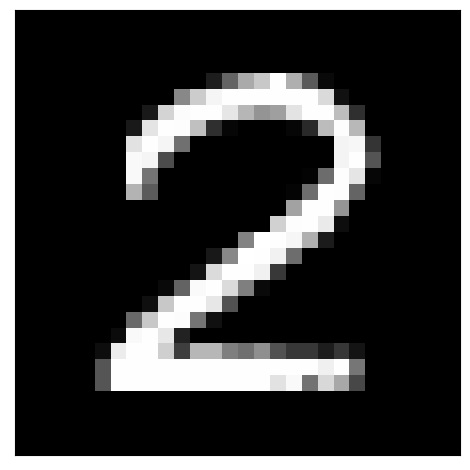
\includegraphics[width=30pt,height=30pt]{Images/mnist_2_0.png}};
%Shape: Square [id:dp3638851328589241] 
\draw   (235.5,162.83) -- (261.5,162.83) -- (261.5,188.83) -- (235.5,188.83) -- cycle ;
%Shape: Triangle [id:dp7565727131335362] 
\draw   (248.5,73.5) -- (261.5,101.5) -- (235.5,101.5) -- cycle ;
%Curve Lines [id:da8502420508886268] 
\draw [color={rgb, 255:red, 74; green, 144; blue, 226 }  ,draw opacity=1 ][line width=1.5]    (259,85.75) .. controls (298,56.5) and (263.8,134.12) .. (299.14,110.21) ;
\draw [shift={(302,108.17)}, rotate = 143.13] [fill={rgb, 255:red, 74; green, 144; blue, 226 }  ,fill opacity=1 ][line width=0.08]  [draw opacity=0] (11.61,-5.58) -- (0,0) -- (11.61,5.58) -- cycle    ;
%Curve Lines [id:da5798459707130834] 
\draw [color={rgb, 255:red, 74; green, 144; blue, 226 }  ,draw opacity=1 ][line width=1.5]    (305.07,105.77) .. controls (337.52,82.6) and (374.55,121.44) .. (412.34,96.43) ;
\draw [shift={(415.25,94.38)}, rotate = 143.13] [fill={rgb, 255:red, 74; green, 144; blue, 226 }  ,fill opacity=1 ][line width=0.08]  [draw opacity=0] (11.61,-5.58) -- (0,0) -- (11.61,5.58) -- cycle    ;
\draw [shift={(302,108.17)}, rotate = 319.74] [color={rgb, 255:red, 74; green, 144; blue, 226 }  ,draw opacity=1 ][line width=1.5]      (0, 0) circle [x radius= 4.36, y radius= 4.36]   ;
%Curve Lines [id:da05644694141454809] 
\draw [color={rgb, 255:red, 208; green, 2; blue, 27 }  ,draw opacity=1 ][line width=1.5]    (266,181.25) .. controls (305,152) and (304.23,193.65) .. (341.24,167.95) ;
\draw [shift={(344.17,165.83)}, rotate = 143.13] [fill={rgb, 255:red, 208; green, 2; blue, 27 }  ,fill opacity=1 ][line width=0.08]  [draw opacity=0] (11.61,-5.58) -- (0,0) -- (11.61,5.58) -- cycle    ;
%Curve Lines [id:da31515691181599714] 
\draw [color={rgb, 255:red, 208; green, 2; blue, 27 }  ,draw opacity=1 ][line width=1.5]    (347.13,163.36) .. controls (377.09,138.62) and (376.31,150.06) .. (412.76,152.43) ;
\draw [shift={(416.25,152.63)}, rotate = 182.6] [fill={rgb, 255:red, 208; green, 2; blue, 27 }  ,fill opacity=1 ][line width=0.08]  [draw opacity=0] (11.61,-5.58) -- (0,0) -- (11.61,5.58) -- cycle    ;
\draw [shift={(344.17,165.83)}, rotate = 319.74] [color={rgb, 255:red, 208; green, 2; blue, 27 }  ,draw opacity=1 ][line width=1.5]      (0, 0) circle [x radius= 4.36, y radius= 4.36]   ;
%Image [id:dp917147005019352] 
\draw (440,60.0) node  {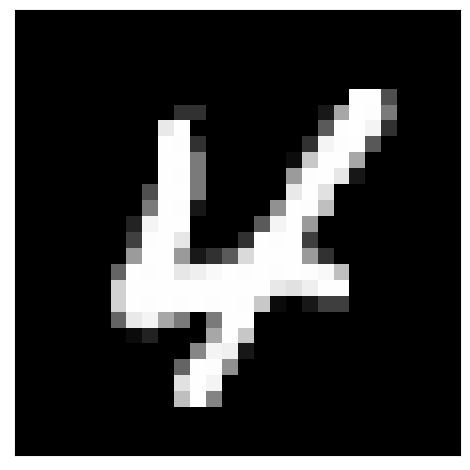
\includegraphics[width=30pt,height=30pt]{Images/mnist_4_1.png}};
%Image [id:dp6739435302515051] 
\draw (440,105.0) node  {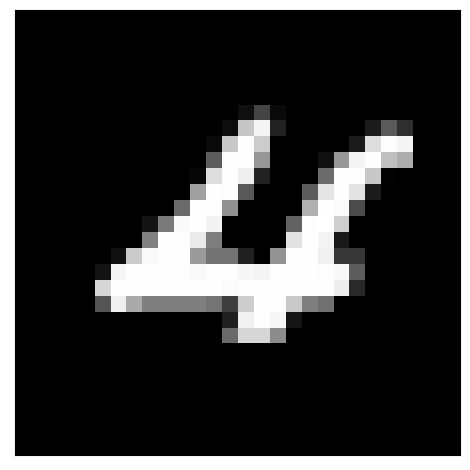
\includegraphics[width=30pt,height=30pt]{Images/mnist_4_2.png}};
%Image [id:dp04932943495314279] 
\draw (440,195.0) node  {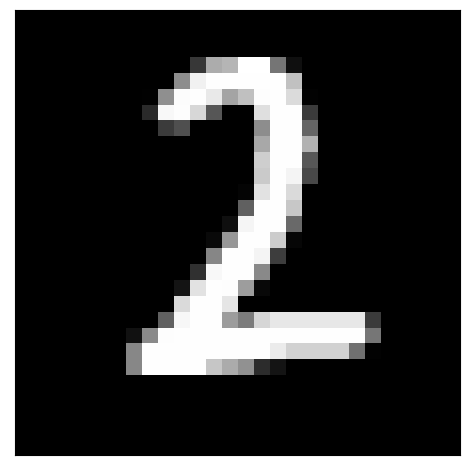
\includegraphics[width=30pt,height=30pt]{Images/mnist_2_1.png}};
%Image [id:dp7844439041624189] 
\draw (440,150) node  {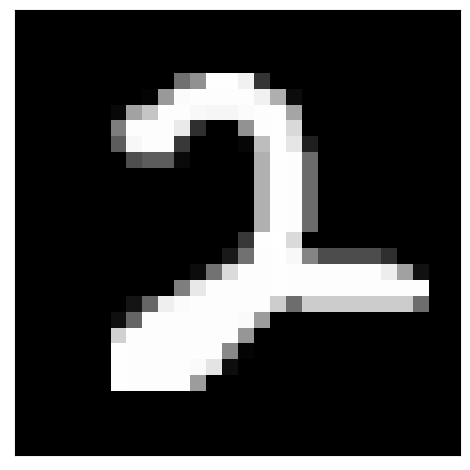
\includegraphics[width=30pt,height=30pt]{Images/mnist_2_2.png}};
\end{tikzpicture}
\caption[Deep similarity encoder]{Visual representation of a deep similarity encoder. Input images (on the left) are mapped to an embedded space (of lower dimension). Images representing the same concept (squares, circles and triangles) are mapped close to each other in clusters. A nearest neighbor search around the embedding of an image will therefore yield similar images. The example images are taken from the MNIST dataset \cite{mnist}. Image inspired by \cite{deep_similarity_encoder}.}
\label{fig:deep_similarity_encoder}
\end{figure}

\section{PSO and distributed attacks}\label{sec:pso_and_distributed_attacks}
There have been several attempts to craft adversarial examples using an \gls{ea}. Previous attempts tried to reduce the number of queries needed to create a successful adversarial example by utilizing \glspl{ea} \cite{genattack,dong2019efficient,mosli2019they,audio_pso,distributed_pso_attack,suryanto2020}. \\

GenAttack \cite{genattack} and the similar efficient attack by Dong et al. \cite{dong2019efficient} use genetic algorithms in order to minimize the number of queries to the model. Both algorithms reduce the dimension of the search space to improve the efficiency of the attack. Once a promising perturbation is found in this lower dimensional space, it is upscaled using a bilinear transformation. By reducing the search space, the number of individuals in the genetic algorithm can be lowered, which in turn lowers the total amount of queries. GenAttack also uses annealing schemes to adaptively scale the parameters of the algorithm. This allows it to escape local optima and improve the adversarial example further. \\

AdversarialPSO \cite{mosli2019they} and the similar attack from \cite{audio_pso} use \gls{pso} as optimization routine on images and audio fragments respectively. Each particle represents a possible adversarial example. Both attacks use the standard rules of \gls{pso} as specified by \cite{pso} improved with a linearly decaying inertia weight \cite{inertia_weight}. The former attack also uses a constriction factor to avoid premature convergence \cite{constriction_factor}. While the latter solves this problem by generating new particles using a genetic algorithm when premature convergence is detected. Both algorithms rely on confidence scores to assign fitness values to certain positions in the search space. \gls{pso}-\gls{bba} \cite{distributed_pso_attack}, is similar to AdversarialPSO, but only relies on distances to determine fitness values. This attack can therefore also be used in decision-based settings instead of solely in score-based settings.\\

The idea behind the multi-group \gls{pso} attack \cite{suryanto2020} is to use multiple \gls{pso} swarms to escape local optima. The intuition behind it is inspired by the \gls{ddos} attack \cite{ddos}. The swarm is split into multiple smaller groups and each group is placed on a single node. The groups perform the standard \gls{pso} algorithm. The best position over all groups is communicated using a dedicated server. Each group submits its queries from its own node, tricking the defensive mechanism into thinking that multiple users are submitting queries. The authors state that this will ultimately result in less detections, but they have not evaluated this against a defensive scheme.\\
